\documentclass[12pt]{article}
\usepackage{url}
\usepackage{hyperref}
\usepackage[utf8]{inputenc}
\usepackage{graphicx}
\usepackage{caption}
\usepackage{float}
\usepackage[left=15mm, right=15mm, top=5mm, bottom=5mm]{geometry}
\usepackage{subcaption}

\title{Are temperatures of one year significantly correlated with next year (sucessive years), in a given location?}

\author{Electric Emus \\ CMEE }

\date{\today}

\begin{document}
  \maketitle
  
    \section{Rationale}

    Serial autocorrelation is when there is significant correlation between successive datapoints in a data set. This means that there is some degree of similarity between the data points where, possibly, exists an unnacounted relationship in one or more of the variables.
    In this report we evaluate the annual mean temperatures from Key West, Florida, USA, between 1901 and 2000. Our aim is to examine this region temperatures fluctuations and analyse if we can detect significant correlation between pair of years.
    
  \section{Methods}

    Data from Key West, Florida climatic region was gathered from the TheMulQuaBio \cite{themulquabio_git} repository. 
    To test for autocorrelation between the data points we have removed one observation from the annual temperature values (n-1) and pair this with its sucessive year.
    We have then calculated the correlation between initial time-points and its sucessive years using Pearsons Correlation (Eq. 1):
    
    \begin{equation}
      \rho = \frac{{}\sum_{i=1}^{n} (x_i - \overline{x})(y_1 - \overline{y})}
      {\sqrt{\sum_{i=1}^{n} (x_i - \overline{x})^2(y_1 - \overline{y})^2}}
    \end{equation}
    
    Following the same process, we have generated random samples of temperatures and iterate this 10,000 times. 
    For each permutation the respective correlation coefficient was calculated.
    To understand the significance of our results we calculate what fraction of our randomized results are greater than the observed initial correlation.

  \section{Results}

  A moderate positive correlation in annual temperatures was found for the initial values $t_0$ and $t_1$  (Figure 1.a). 
  This same autocorrelation was not seen in the permutated simulations that we ran. 
  Figure 2.b represents the frequency of this correlations generated, with most of coefficients falling between negative (-0.2) and positive (0.2) weak correlations.
  The fraction of randomized permutations that have the same correlation of initial values was very low, being significantly different ($ P\textsubscript{value} < 0.001 $).



    \begin{figure}[H]
      \centering
      \begin{subfigure}{.45\textwidth}
        \captionsetup{singlelinecheck = false, format = hang, justification = raggedright, font = footnotesize, labelsep = space}
        \centering
        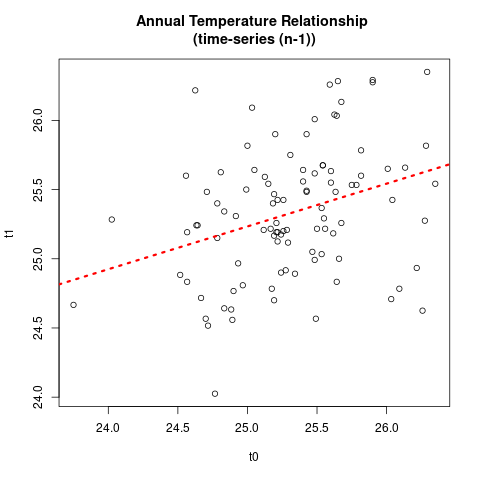
\includegraphics[width=1\linewidth]{../results/Florida_Temperatures_relationship.png}
        \caption{Relationship between observed $t_0$ and $t_1$ Temperatures for Key West Florida}
        \label{fig:sub1}
      \end{subfigure}
      \begin{subfigure}{.45\textwidth}
        \captionsetup{singlelinecheck = false, format = hang, justification = raggedright, font = footnotesize, labelsep = space}
        \centering
        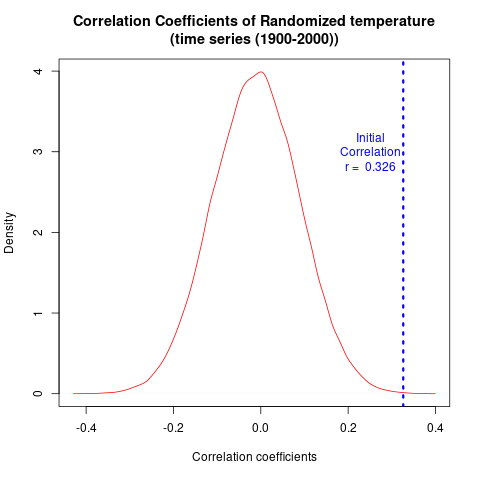
\includegraphics[width=1\linewidth]{../results/Florida_Temperatures_cor_density.png}
        \caption{Frequency of correlation coefficients for the 10,000 permutations}
        \label{fig:sub2}
      \end{subfigure}
      \caption{Scatterplot and density plot of Key West}
      \label{fig:test}
    \end{figure}


  \section{Discussion}

  The goal of our mini report was to identify any potential serial autocorrelation between observed data points.
  Despite the evidence mounting for an increase in temperatures across the globe, our randomized sampling does not follow this pattern, resulting in a significant correlation different from the initial observations.
  Nevertheless, being Florida located in a region that it is potentially threathened by climate change adverse events, our exhaustive randomized simulations did not detect any inflated behaviour in the data points that might suggests an increase in temperarures over diferent time-series.


  \bibliographystyle{apalike}
  \bibliography{TAutoCorr}
   
\end{document}